\subsection{闭映射特有的性质}

命题 9. 设 X、X' 是两个拓扑空间。映射 \(f: \mathbf{X} \to \mathbf{X}'\) 连续且闭的充分必要条件是：对 X 的每个子集 A，\(f(\overline{\mathbf{A}}) = \overline{f(\mathbf{A})}\)。

该条件是充分的，因为它显然蕴含 \(f\) 是闭映射，且由 § 2 第 1 目定理 1，它也蕴含 \(f\) 连续。反之，若 \(f\) 连续且闭，则由 § 2 第 1 目定理 1，我们有 \(f(\mathbf{A}) \subset f(\overline{\mathbf{A}}) \subset \overline{f(\mathbf{A})}\)；又按假设 \(f(\overline{\mathbf{A}})\) 在 \(\mathbf{X}'\) 中是闭集；从而 \(f(\overline{\mathbf{A}}) = \overline{f(\mathbf{A})}\)。

命题 10. 设 R 是拓扑空间 X 上的一个等价关系。则 R 是闭的，当且仅当模 R 的每个等价类 M 都具有由关于 R 饱和的邻域组成的一个基本邻域系。

设 R 是闭的，并设 U 是 M 的任一开邻域；由于 \(F = \complement U\) 在 X 中是闭集，F 关于 R 的饱和化 S 在 X 中是闭集。由于 M 关于 R 是饱和的，我们有 \(M \cap S = \varnothing\)，从而 \(V = \complement S\) 是 M 的一个开邻域，它关于 R 饱和且含于 U。

为证其逆，设 F 是 X 的任一闭子集。设 T 是 F 关于 R 的饱和化，设 x 是 \(\complement T\) 的一点，并设 M 是 x 的等价类；则 \(M \cap T = \varnothing\)，从而更有 \(M \cap F = \varnothing\)，于是 U = \(\complement F\) 是 M 的一个邻域。因此存在 M 的一个邻域 \(V \subset U\)，使 V 关于 R 饱和；V 不与 F 相交，故不与 T 相交，从而 \(\complement T\) 是 M 的、因而是 x 的一个邻域。这表明 \(\complement T\) 是开集（§ 1，第 2 目，命题 1），亦即 T 是闭集。

注. 命题 10 蕴含以下事实：若 R 是闭的，且用 \(\varphi\) 表示典范映射 \(X \to X/R\)，则对每个 \(x \in X\) 以及 \(x\) 的等价类在 X 中的每个邻域 U，\(\varphi(U)\) 都是 \(\varphi(x)\) 在 X/R 中的一个邻域。应当仔细注意，这一断言决不蕴含：对 \(x\) 的每个邻域 V，\(\varphi(V)\) 都是 \(\varphi(x)\) 的邻域；换言之（第 3 目，命题 5），闭等价关系未必是开的（习题 2）。反过来，开等价关系也未必是闭的（第 1 目，例 4）；

\pandocbounded{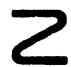
\includegraphics[keepaspectratio]{images/part001_bfecd507.jpg}}

因为若 U 是某个等价类 M 在 X 中的一个邻域，则对每个 \(x \in M\) 以及 x 的每个邻域 \(V \subset U\)，V 的饱和化固然是 M 在 X 中的一个邻域，但这个邻域未必含于 U。

最后，存在除相等关系之外既开又闭的等价关系（习题 3），也存在既不开又不闭的等价关系（\(§\ 8\)，习题 10）。

